\documentclass[a4paper,10pt]{article}

\usepackage[a4paper, total={6in, 9in}]{geometry}
\usepackage[utf8]{inputenc}
\usepackage{amsmath}
\usepackage{amsfonts}
\usepackage{graphicx}
\usepackage[ruled,vlined]{algorithm2e}
\usepackage{hyperref}
\usepackage{cleveref}
\usepackage{color}
\usepackage{subcaption}
\usepackage{verbatim}
\usepackage{minted}


\author{Harry Tzovas}

\definecolor{blue1}{RGB}{44,127,184}

\newcommand{\wave}{$\mathcal{WAVE}$ }
\newcommand{\geo}{\textsc{Geographer} }
\newcommand{\bull}{$\bullet$}
\newcommand{\red}[1]{{\color{red}{#1}}}
\newcommand{\blue}[1]{{\color{blue1}{#1}}}
\newcommand{\mz}{\mathbb{Z}}
\newcommand{\quot}[1]{``#1''}
\newcommand{\km}{$k$-means}
\newcommand{\etc}{e.t.c.}
\newcommand{\todo}[1]{{\red{TODO}}: #1}
\newcommand{\att}{\textbf{Attention}: }
\newcommand\noIndent[1]{
  \par\vbox{\parbox[t]{\linewidth}{#1}}
}
\newcommand{\MI}[1]{\mintinline{c++}{#1}}


\graphicspath{{/home/harry/wave/figures/}{/home/harry/geographer-dev/figures/}}



\begin{document}


\section*{Contributing to Geographer}

This section describes in some depth some of the lama and \geo data types and functionality intended
mainly for anyone that wants to contribute to the project. We will take a look into the commonly
used data type and how to use them efficiently.

\subsection*{Lama}

Lama is a framework for developing hardware-independent, high performance code. It offers distributed 
data types, like DenseVector or CSRSparseMatrix, and simplified functions that might include communication
between processing elements (PEs) underneath. What it might be intricate code when writing raw MPI code,
it becomes a simple function call. Below, we will see some of the most used data structures and 
functions in \geo.


\subsubsection*{Distribution}

%As we have seen, matrices and vectors are distributed among PEs.
In high performance application, data are usually too large to fit in a single memory plus, for
better running time, we use distributed data. For example, vectors that are distributed among several
memory units. Since each PE owns only a part of the data, we distinguish between \emph{local} 
and non-local data. We also have to keep in mind how indexing is done, Typically, the element
of a distributed vector has two related indices, its local index referring to its position
to the local vector, and a global index that is its position relevant to the global vector.
A distribution can be defined as a mapping from the local to global indices and vise versa.

The simplest way to distribute data
is the \MI{scai::dmemo::BlockDistribution}. Say that the size of the data to be distributed is $n$
(either this is the size of a \MI{DenseVector} or the number of rows of a matrix) and we want
to distribute them among $p$ PEs. Using a \MI{BlockDistribution} each PE will own $\lfloor n/p \rfloor$
consecutive elements and PE $i$ will own indices from $i\lfloor n/p \rfloor$ until $(i+1)\lfloor n/p \rfloor$,
with the last PE possibly having more elements.

A more flexible version is the \MI{scai::dmemo::GenBlockDistribution} where again each PE owns a 
consecutive list of indices but now the size of the elements that belong to each PE can vary.

In the other extreme is \MI{scai::dmemo::GeneralDistribution} which allows any arbitrary distribution
of indices. If you notice, the rows of the matrix in \cref{fig:graph} are distributed using a
\MI{GeneralDistribution}. 

In \cref{fig:dist} you can see a vector of 14 elements divided among 3 PEs using 3 different 
distributions. A functional difference between distributions is how to find which PE owns a given
index $i$. For the \MI{BlockDistribution} and the \MI{GenBlockDistribution} this is easy and each
PE can calculate fast the owner of $i$. This is much more costly for the \MI{GeneralDistribution} 
since $i$ can be anywhere and communication among PE is needed.
For this, there is an optimized version \MI{computeOwners()} that returns the owners for a given array of 
global indices. Similarly, the function \MI{local2Global()} and \MI{global2Local()} are more expensive
for a general distribution compared to a block distribution.


\subsubsection*{CSR sparse matrix}

The data structure to store the graph is a distributed CSR sparse matrix\footnote{\url{https://en.wikipedia.org/wiki/Sparse_matrix}} 
\begin{minted}{c++}
scai::lama::CSRSparseMatrix
\end{minted}

%Every distributed matrix can have one distribution for its rows and one for its columns,
%that is, in which PE each element belongs to. We say that a PE \emph{owns} an element or a row
%and that an element or a row \emph{belongs} to a PE. Often, each element of the matrix belongs only to one PE.
In a distributed matrix, there are two possible distributions of its elements to the available
PEs; one along the rows and one along the columns of the matrix.
Such distributions define assignments of elements to PEs. We say that a PE \emph{owns} an element or a row
and that an element or a row \emph{belongs} to a PE. Often, each element of the matrix belongs only to one PE.
Here, when using the distributed matrix to store the adjacency matrix of a graph, we use only a distribution 
along the rows. So, the rows of the matrix are divided among PEs, and each row exists only in one PE.
In graph theoretic term, this is equivalent to saying that each PE owns a subset of the vertices (since
one row corresponds to one vertex of the graph) and knows the neighbors of every vertex. 
So for the rest, a vertex of the matrix and a row of the matrix are equivalent.
One example of a distributed graph (and matrix) can be seen in \cref{fig:graph}.

\begin{figure}[h]
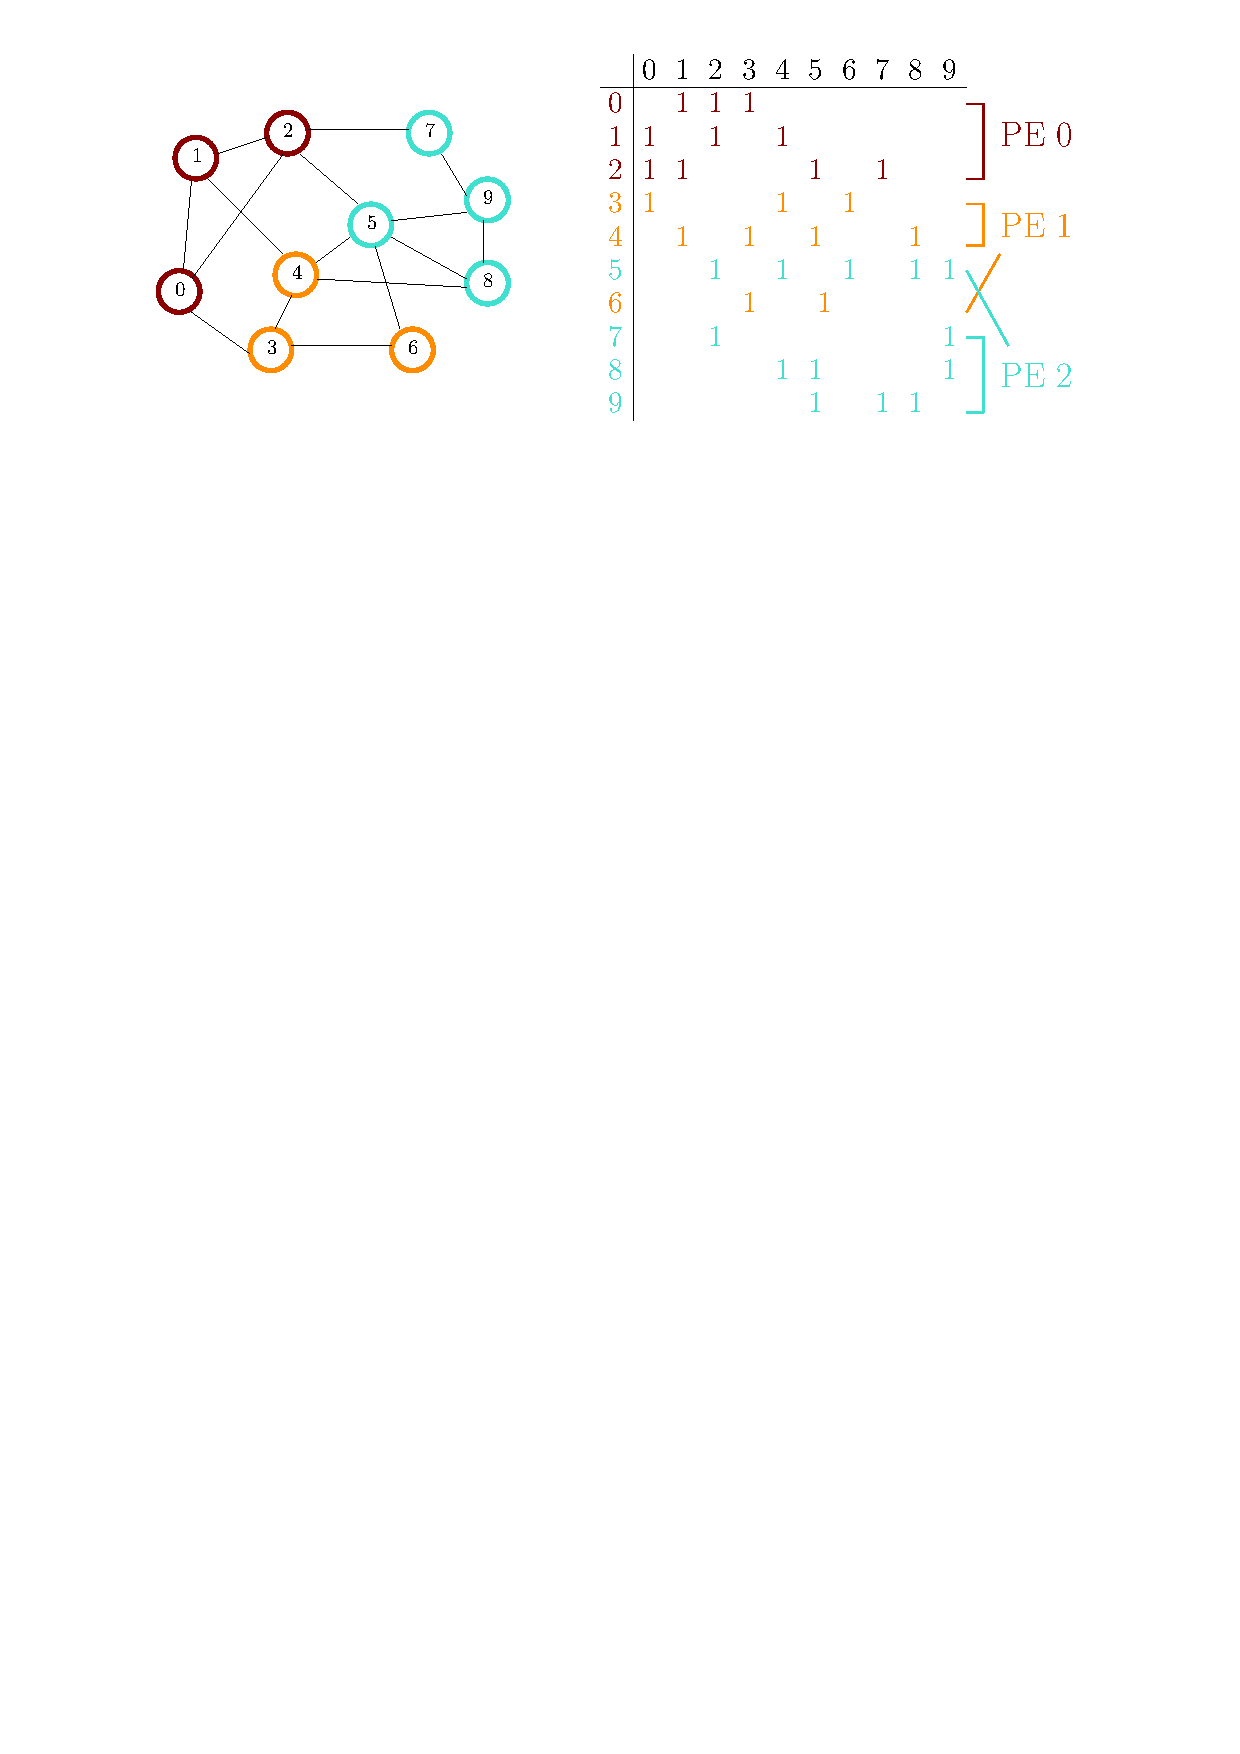
\includegraphics[scale=0.9]{graph}
\caption{A graph with 10 nodes distributed among 3 PEs and the corresponding distribution of the 
adjacency matrix. \att this is not a partition in the theoretical sense, just a distribution of
the rows of the matrix.}
\label{fig:graph}
\end{figure}

The CSR sparse matrix format uses three vectors to store the matrix and in the distributed case
these vectors are distributed among PEs. Since each PE owns a part of the matrix,
we distinguish between \emph{local} and non-local data. Also, PEs have access to some global information 
such as the global size of the matrix, the row and column distribution \etc. 

For convenience, there are functions that hide these details from the user.
For example, the function \mintinline{c++}{CSRSparseMatrix::getValue(i,j)} returns the value 
in position $[i,j]$
of the matrix. But indices $i$ and $j$ refer to the global indexing, that is, if matrix has dimensions
$N\times N$ then $0\leq i,j < N$; but position $[i,j]$ exists only in a single PE. When getValue() is
called, every PE checks if it owns this position, the one PE that owns it accesses the data and 
then it broadcasts the value to all PEs. So, using functions like that make it easier to write code
but it can hide, possibly, unnecessary communications.

To avoid communication cost (so to be efficient!), we want, most of the times, to access only local 
data. To make this explicit, we retrieve the local data of the matrix. 
This is done using \mintinline{c++}{scai::lama::SparseMatrix::getLocalStorage()}. 
Through the localStorage we can then read or write the local values without worrying about unwanted 
communications. To read and write we need to acquire a lock to the data; this is done via the
\mintinline{c++}{scai::hmemo::ReadAccess} and \mintinline{c++}{scai::hmemo::WriteAccess}

\att Because of the structure of the CSR sparse matrix, for an already initialized matrix, we can only 
change already existing values. If position $[i,j]$ does not exist, i.e., is zero, then we cannot 
access it directly and we need to adapt the CSR vectors directly.

A reoccurring pattern of code to access the data of the adjacency matrix is in \cref{alg:csrData}.
after line \ref{code:csr1} until line \ref{code:csr2}. Along with the 2 for loops, is a common way to
access all local edges. 
By getting the distribution pointer, line \ref{code:dist}, we can check if a global index is local 
in this PE or not.
The function to do that is \MI{scai::dmemo::Distribution::isLocal(i)} and to convert local
indices to global and vise versa, there are function
\MI{scai::dmemo::Distribution::local2Global(i)} and \\
\MI{scai::dmemo::Distribution::global2Local(i)}.

\att  for \MI{isLocal} and \MI{global2Local}, index $i$ is taken as a global index, i.e., $0\leq i <N$; this last function returns a specific number (\texttt{invalidIndex})
if the requested index is not local. Similarly, for \MI{local2Global(i)} $0\leq i < localN$.
Naturally, \MI{isLocal(i)} is true in only one PE and false at the rest.

For example, for \cref{fig:graph}, \mintinline{c++}{isLocal(4)} is true only for PE 1, 
\mintinline{c++}{global2Local(7)} will return 1 for PE 2 and \texttt{invalidIndex} for PE 0 and 1 and
\mintinline{c++}{local2Global(1)} will return 1 for PE 0, 4 for PE 1 and 7 for PE 2.

%
\begin{algorithm}[h]%
\begin{minted}[tabsize=4, linenos, mathescape]{c++}
std::vector<IndexType> GraphUtils::nonLocalNeighbors(
	const CSRSparseMatrix<ValueType>& graph){ 

	//get the distribution of the rows
	//will be used to determine if an index is local or not $\label{code:dist}$
	const scai::dmemo::DistributionPtr inputDist = graph.getRowDistributionPtr();
	
	// access local data $\label{code:csr1}$
	using scai::hmemo::ReadAccess;
	const CSRStorage<ValueType>& localStorage = graph.getLocalStorage();
	const ReadAccess<IndexType> localIa(localStorage.getIA()); //local ia
	const ReadAccess<IndexType> localJa(localStorage.getJA()); //local ja
	const ReadAccess<ValueType> localValues(localStorage.getValues());
	//^^^ not needed for this example, just for illustration purposes $\label{code:csr2}$
	
	//local number of vertices/rows
	const IndexType localN = graph.getLocalNumRows(); 
	
	//since this allows duplicates,  we count edges
	std::multiset<IndexType> neighborSet; 
	
	//for all local vertices
	for (IndexType i=0; i<localN; i++) {
		//range of this vertex's neighbors
		const IndexType beginCols = localIa[i];
		const IndexType endCols = localIa[i+1];
		
		//for all neighbors of this vertex
		for (IndexType j=beginCols; j<endCols; j++) {
			//since there is no column distribution, neighbor is the global id
			IndexType neighbor = localJa[j];
			
			//insert only if neighbor is not in the same PE
			//isLocal() is constant for block and general block distributions
			//but log(localN) for a general distribution
			if( !inputDist->isLocal(neighbor) ){
	        	neighborSet.insert(neighbor);
	        }
		}
	}	
	return std::vector<IndexType>(neighborSet.begin(), neighborSet.end()) ;
}
\end{minted}
\caption{Code to get all the non-local neighbors for every vertex. Every PEs goes over only its local
data. Of course, the returned vectors will be different for every PE.}
\label{alg:csrData}
\end{algorithm}


The function in \cref{alg:csrData} will return a vector with the global ids of all the vertices 
that are connected to some local vertex but themselves belong to other PEs.
This is called the \emph{halo} of the PE. For example, in \cref{fig:graph}, the halo of PE 0
are the vertices $3, 4, 5$ and $7$.

Lama offers the \MI{scai::dmemo::HaloExchangePlan} class to store info about the halo 
exchange between PEs. In \cref{alg:halo} you can see a short example of how to build and access 
the halo of a graph. 
Function \MI{HaloExchangePlan::updateHalo()} includes communication between PEs as it
will send and receive the appropriate data for each PE according to its halo.
For the graph in \cref{fig:graph}, PE 0 will send the values of \MI{partition[0]} and \MI{[1]}
to PE 1 and \MI{partition[2]} to PE 2 and will receive \MI{partition[3]} and \MI{[4]} from
PE 1 and \MI{partition[5]} and \MI{[7]} from PE 2. Since data in the halo are stored with their
global ID, to access it we need to map the global index to the relative index of our halo.
This is done by calling \MI{HaloExchangePlan::global2Halo(i)} (there is also the inverse,
to get the global position of a halo index by \MI{HaloExchangePlan::halo2Global(i)}).

\begin{algorithm}
\begin{minted}[tabsize=4, linenos, mathescape]{c++}

// given a dense vector that stores a partition of the graph as
// scai::lama::DenseVector<IndexType> partition

// get the local data of the partition
const scai::hmemo::HArray<IndexType>& localPart= partition.getLocalValues();

// get the global IDs of halo vertices
// where graph is a scai::lama::CSRSparseMatrix<ValueType>
scai::dmemo::HaloExchangePlan partHalo = 
	ITI::GraphUtils<IndexType,ValueType>::buildNeighborHalo( graph );

// get the value from the partition for all the halo vertices
// comm is the communicator: scai::dmemo::CommunicatorPtr
scai::hmemo::HArray<IndexType> haloData;
partHalo.updateHalo( haloData, localPart, *comm );	

// now, haloData stores the value of the partition vector for all
// the halo vertices. To access the data in similar for loop as in $\cref{alg:csrData}$
//...
//for all local vertices
for (IndexType i=0; i<localN; i++) {
	//range of this vertex's neighbors
	const IndexType beginCols = localIa[i];
	const IndexType endCols = localIa[i+1];
	for (IndexType j=beginCols; j<endCols; j++) {
		IndexType neighbor = localJa[j];
		// the block id in which the neighbor belongs to
		IndexType neighborBlock = haloData[partHalo.global2Halo(neighbor)];
//...
\end{minted}
\caption{Get and access the halo data of DenseVector partition.}
\label{alg:halo}
\end{algorithm}


\subsubsection*{DenseVector}

The other commonly used data structure is the \MI{scai::lama::DenseVector} which is a vector distributed
among PEs by some distribution. By calling \MI{DenseVector::getLocalValues()} we get only the part
of the vector owned by the process and we can process the local data without worrying about hidden
communications. In \cref{alg:vector} we access the local data of dense vector and copy them to 
a \MI{std::vector} if, for example, we want to call some standard function like sorting.

\begin{algorithm}
\begin{minted}[tabsize=4, linenos, mathescape]{c++}
//where partition is an input vector given as
// const DenseVector<IndexType> &partition
scai::hmemo::ReadAccess<IndexType> partAccess( partition.getLocalValues() );
std::vector<IndexType> neighborPEs( 
	partAccess.get(), partAccess.get()+partAccess.size() );
\end{minted}
\caption{Code to store the local data of a distributed DenseVector to a \MI{std::vector}}
\label{alg:vector}
\end{algorithm}

For example, we are using \MI{std::vector<DenseVector<ValueType>> partition} to store a partition of the graph
into blocks as in \cref{alg:halo,alg:vector}. If \MI{partition[i]=x}, this means that vertex \MI{i}
is in block \MI{x}.
The \MI{partition} vector has the same size as the 
dimension of the matrix but should also have the same distribution as the row distribution of the matrix.


\begin{figure}
\centering
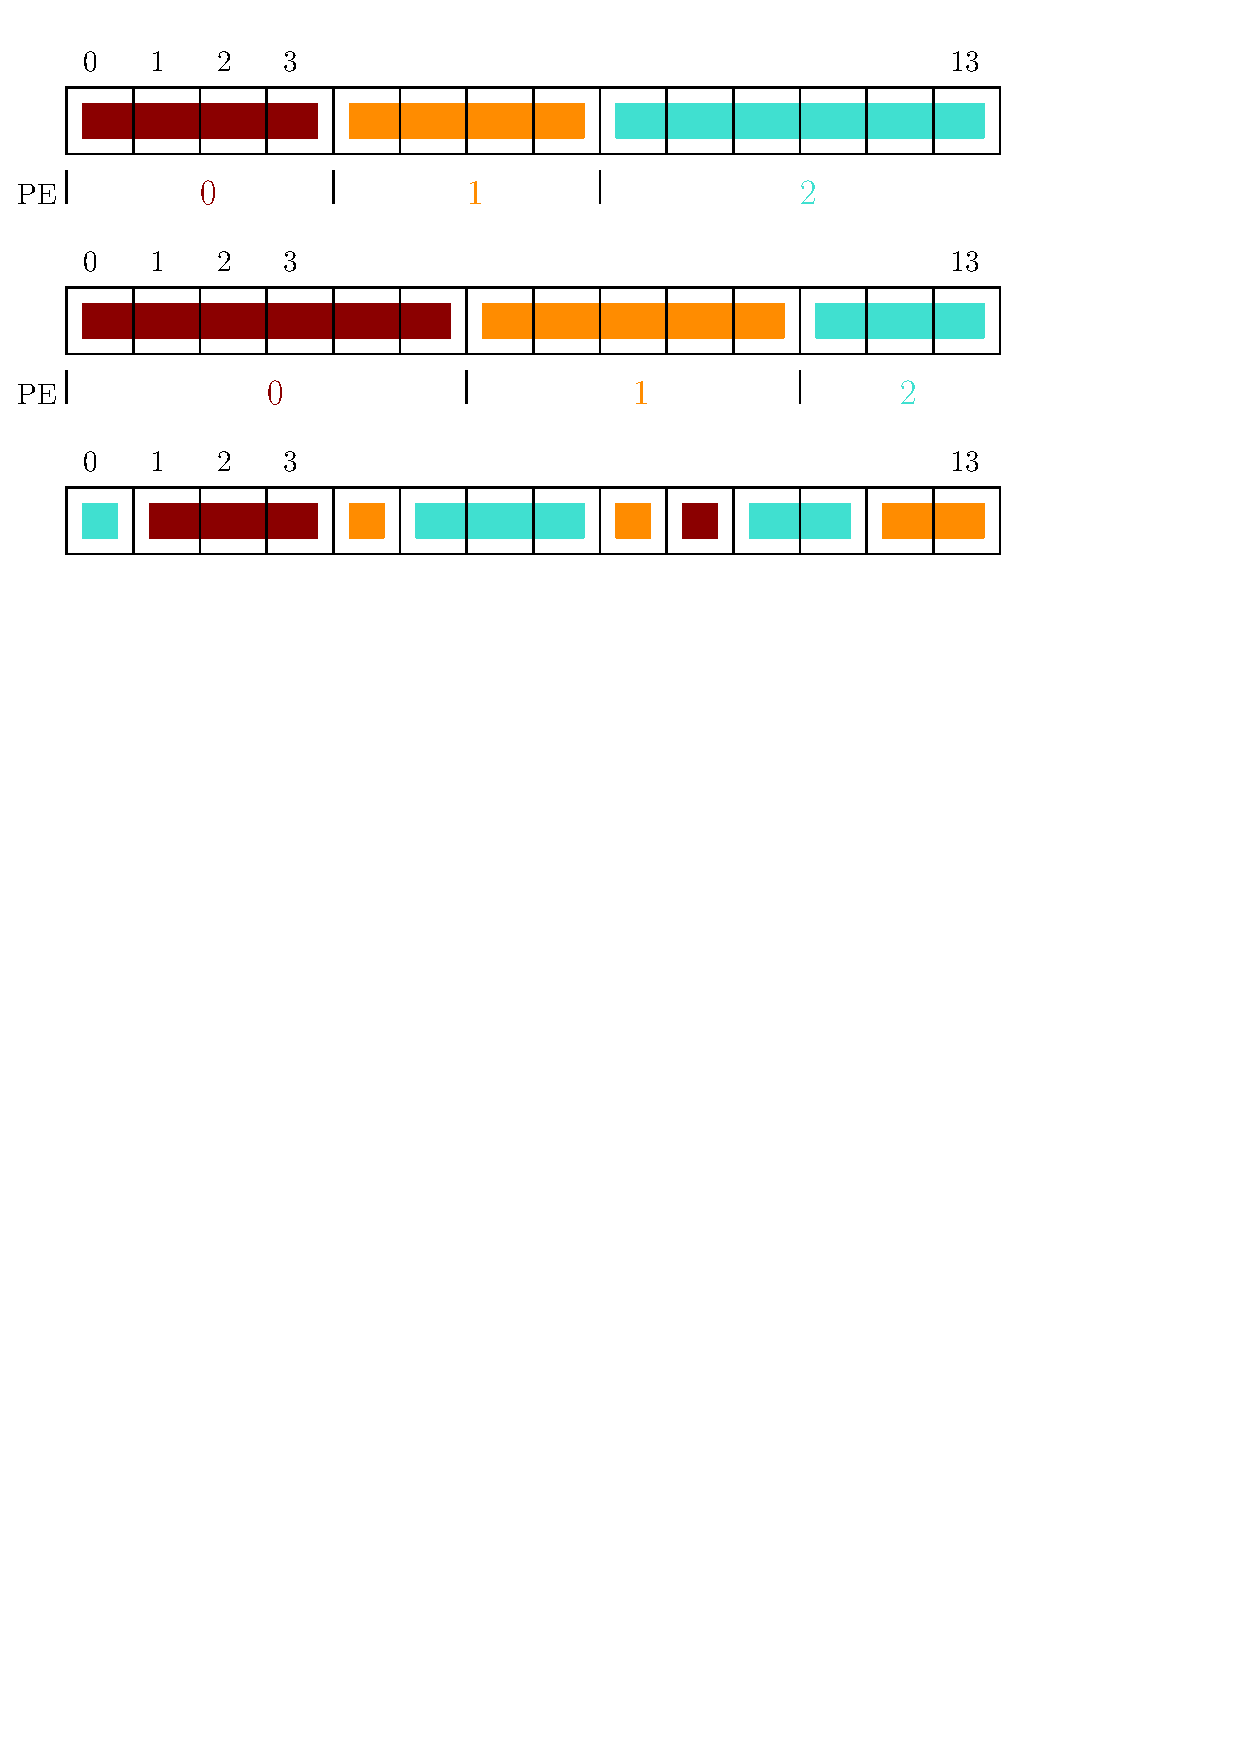
\includegraphics[scale=0.7]{vector_dist}
\caption{A block distribution, a general block distribution and a general distribution of a vector
with 14 elements.}
\label{fig:dist}
\end{figure}

Some useful function for all distributions are \MI{getLocalSize()} and \MI{getGlobalSize()} that return
the local and global size of the distribution, \MI{getCommunicator()} that returns the communicator associated
with this distribution and \MI{isEqual()} to test if two distributions are equal.


\subsubsection*{Communicator}

Every distribution uses a \MI{scai::dmemo::Communicator} object. Communicators are needed for 
data exchange between different PEs of a distributed application. They support all usual functions
of an MPI communicator. Some of the most commonly used functions 
of a communicator are \MI{getRank()} and \MI{getSize()} that return the PE id of the calling PE and the
total number of PEs respectively; \MI{min(x)} and \MI{max(x)} return the min and max of a
number $x$ among all PEs. \MI{sum(x)} returns the sum of $x$ among all PEs; for that all $x$'s are sent to one PE, the
sum is calculated there locally and then it is broadcasted to all PEs. Similarly, \MI{sumImpl()}
calculates the sum of a vector; note that this vector is not distributed, every PE \quot{contributes}
local data.

\clearpage


\subsection*{Geographer }

In this section we present some useful functions and what should be adapted within \geo if you want 
to contribute to the project.
By design, the main \quot{entry point} for a new algorithm is \MI{ITI::ParcoRepart::partitionGraph()}, which
is the function to call if you want to partition a graph or a point set. 
For most (overloaded) versions of \MI{partitionGraph()}, 
the input typically consists of 3 objects: a \MI{CSRSparseMatrix} that is the adjacency matrix of the
graph, a \MI{std::vector<DenseVector<ValueType>>} that is used to store the coordinates of the vertices
and a \MI{DenseVector} to store the weights of the vertices.
For those more familiar with metis and parmetis, there is also a version that takes raw pointers and
internally converts them to \MI{CSRSparseMatrix} and \MI{DenseVector} and then calls the core implementation
of \MI{partitionGraph()}. The arguments of this version are the same (or similar) to the metis and
parmetis prototypes.
By using the \MI{Settings} struct you can choose which algorithm you want to use for partitioning and
pass various input parameters to the partitioning algorithm.

If you want to contribute a new partitioning algorithm
you should first create a separate class, add a value in \MI{Settings::Tools} and  adapt the 
\MI{ITI::ParcoRepart::partitionGraph()} function in order to call the desired partitioning function.
The core implementation of \MI{partitionGraph()} is separated in two main parts: 
first we get the initial partition of a graph or point set and then we do local refinement using 
the multilevel scheme. 
The first part can be found in \MI{ParcoRepart::initialPartition()}; this is where you most probably
want to add the call to the new function. Afterwards, applying
local refinement can improve the cut provided by your algorithm.
By setting \MI{Settings.noRefinement} to true, local refinement is disabled.
Any required input parameter for the new algorithm should be declared in \MI{Settings}.
Probably, you must also adapt \MI{parseArgs} so the parameters can be passed at run time as 
command line arguments.

\att in the case that you algorithm is about local refinement you should probably do more extensive
changes as currently we do not support different local refinement algorithms.

Useful helper functions for graph and points sets can be found in \MI{ITI::aux}
and \MI{ITI::GraphUtils}. For example, in \MI{GraphUtils} there are function to compute the cut, the imbalance,
the diameter of blocks and other properties of a partitioned (or not) graph. You can also construct the 
communication and processor graph. The communication graph has a vertex for each block and two vertices
are adjacent if and only if the blocks are adjacent. The processor graph does not require the graph
to be partitioned; a vertex of the processor graph corresponds to a PE and two vertices are adjacent 
if the local data in the respective PEs have adjacent vertices. An example can be seen in
\cref{fig:part_graph}. You can also get an edge coloring of a graph,
construct its laplacian matrix, convert a an adjacency matrix to an edge list \etc.
Another useful function is \MI{aux::redistributeFromPartition()} that, given a partition of the graph 
it redistributes the input (graph, coordinates and node weights) according to that partition.
Many functions to read and write graphs and coordinates from and to files can be found
in the \MI{ITI::FileIO} class.

\begin{figure}[h]
\centering
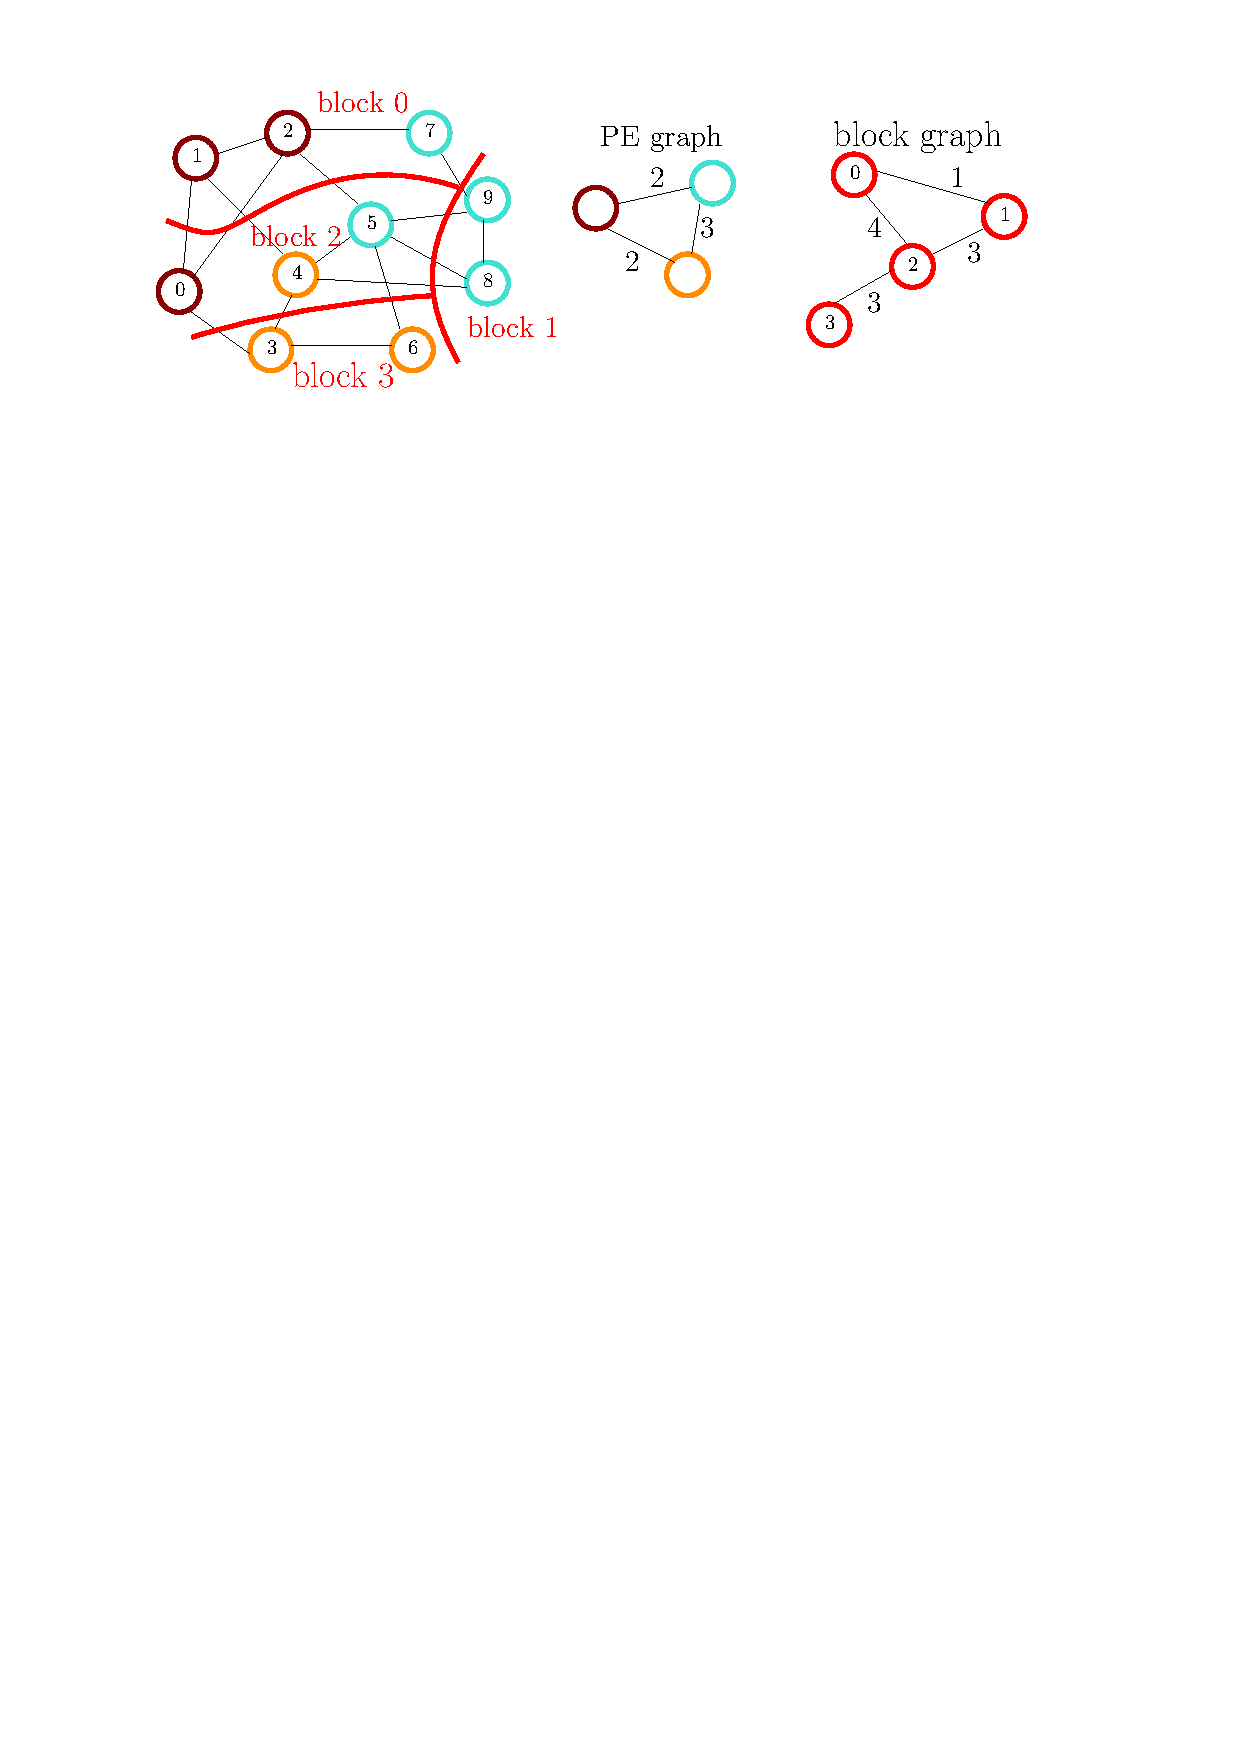
\includegraphics[scale=0.9]{graph_partitioned_with_PE_block_graph}
\caption{A distributed graph between 3 PEs and partitioned to 4 blocks. Different colors indicate the PEs
and red lines indicate the partition. In the middle is the communication graph and on the right the
block graph with the weights on the edges.}
\label{fig:part_graph}
\end{figure}

Apart from the above, to get the geometric partition of a point set there are classes \MI{ITI::KMeans},
\MI{ITI::HilbertCurve} and \MI{ITI::MultiSection}. These classes can partition weighted point sets in the given
number of blocks adhering to a given balance constrain. To do so, each class provides a 
\MI{computePartition} function with similar prototypes. To see how to control the parameters for
each class look into \MI{Settings}. Although some of them require also the
graph, this is mainly for sanity checks and debugging reasons and only the geometric information,
i.e., the coordinates,
are used. In the \geo workflow, a mesh is first partitioned using one of the above techniques and
then is further refined using the graph.

\att some of this function internally redistribute the input data in order to improve locality of the
point and reduce running time. For example, before calling the balanced \km algorithm we redistribute
the input using \MI{HilbertCurve::redistribute} that redistributes the points according to their
hilbert space filling curve (SFC) indices. Look into the documentation of each class for more details.

The classes \MI{MultiLevel} and  \MI{LocalRefinement} are used to coarsen the graph using the
multilevel scheme and apply local refinement, i.e., move vertices between blocks only if moving
the vertex improves the cut value without hurting the imbalance.
Usually, when using the multilevel approach, we start with a non-partitioned graph and merge vertices
together until we reach a small number of vertices. Then this graph is partitioned. To improve
the cut we then refine the coarsen graph and do local refinement. The approach in \geo is different.
Although the uncoarsening/refinement step is identical, for the coarsening step we start from an
already partitioned graph, the one provided by the geometric partition. To merge vertices we
use a matching algorithm that only matches two adjacent vertices if they belong to the same block.
This means that cut edges (edges between blocks) are not considered in the matching and so, the cut 
value of the initial partition and the coarsest graph should be equal.

To do a local refinement to a partitioned graph call \MI{ITI::MultiLevel::multiLevelStep()}. 
This function will do the coarsening and uncoarsening and internally, while uncoarsening,
will do the local refinement.

\att currently, local refinement only works when $k=p$, i.e., the number of desired blocks and the
number of PEs are the same. Additionally, vertices are actually moved between PEs. That means
that the input graph must be redistributed according to the given partition before the local refinement
(here, \MI{aux::redistributeFromPartition()} can be helpful)
and that vertices are redistributed during the local refinement.

If you have an already partitioned graph and you want to repartition/rebalance it you can do
so by setting \MI{settings.repartition} to true and call \MI{ParcoRepart::computePartition()}.
If repartition is activated, internally we call the function \MI{KMeans::computeRepartition()}.
You can also call this function directly to repartition a point set.

\subsubsection*{Example: contribute a new partitioning algorithm}

Suppose that you have designed a new algorithm to partition a graph called \MI{MyAlgo}
and the implementation of the algorithm is in the files MyAlgo.cpp and MyAlgo.h. Two example files
can be seen in \cref{MyAlgo.h} and \cref{MyAlgo.cpp}.
The prototype of the partitioning function should look something like
\begin{minted}{c++}
MyAlgo::partitionGraph( 
    CSRSparseMatrix<ValueType>& graph,
    std::vector<DenseVector<ValueType>>& coordinates,
    std::vector<DenseVector<ValueType>>& nodeWeights,
    struct Settings settings,
    struct Metrics& metrics);
\end{minted}

Note that the function name can be anything, it does not have to be \MI{partitionGraph}. Another 
possibly useful argument can be a \MI{ITI::CommTree} that is used to store the processor
graph, i.e., the physical network, and can be taken into account while partitioning. Of course,
the function can have less input arguments.


\att you must force instantiation of the class otherwise you will get linking error.
One way to do it is to add the line 
\begin{minted}{c++}
template class MyAlgo<IndexType, ValueType>;
\end{minted}
within namespace ITI in file MyAlgo.cpp.

In order to call \MI{MyAlgo} to get the initial partition you should first add an entry to enum
\MI{Settings::Tool} in Settings.h,
called for example \MI{MyAlgo} and add the tool in the \MI{operator<<} and \MI{operator>>} in
Settings.cpp.
Then adapt the code in \MI{ParcoRepart::initialPartition()} to call \MI{MyAlgo::partitionGraph}. 
To do that, you should set the \MI{Settings.initialPartition}
variable that is checked within \MI{initialPartition()} and determines the algorithm to be used.
Maybe you want to add some parameters used by the algorithm. These should be added in Settings.h.
In this case, you must adapt the \MI{ITI::populateOptions} in \MI{parseArgs}; probably you want also 
to add some sanity checks for the new input parameters.

After initial partition, applying local refinement can improve the cut provided by your algorithm. 
If you do not want that you must set \MI{Settings.noRefinement} to true and local refinement is disabled.
To test the behavior and correctness of \MI{MyAlgo} class you should also write a unit test,
typically in a file called MyAlgoTest.cpp. For testing we are using the googletest framework.
To get various metrics of a partitioned graph (that can be useful for sanity checks) you can
use the \MI{Metrics} class or separate function located in \MI{GraphUtils}.

Finally, you should add the MyAlgo.* files in the src/CMakeLists.txt file under FILES\_HEADER for the
.h file, FILES\_COMMON for the .cpp file and FILES\_TEST for the test file.


\begin{algorithm}
\begin{minted}{c++}
#pragma once
#include <scai/lama.hpp>
#include <scai/dmemo/Communicator.hpp>
#include "Settings.h"

namespace ITI {
	
using namespace scai::lama;

/** @brief Main class to partition a graph using new algorithm MyAlgo.
*/

template <typename IndexType, typename ValueType>
class MyAlgo {
public:
    /** Documentation
     */
    static DenseVector<IndexType> partitionGraph(
        CSRSparseMatrix<ValueType> &input,
        std::vector<DenseVector<ValueType>> &coordinates,
        std::vector<DenseVector<ValueType>> &nodeWeights,
        struct Settings settings,
        struct Metrics& metrics);
	
	// other functions in the class
	
}; //MyAlgo
}  //ITI
\end{minted}
\caption{File MyAlgo.h}
\label{MyAlgo.h}
\end{algorithm}

\begin{algorithm}
\begin{minted}{c++}
#include "MyAlgo.h"

namespace ITI {
	
template<typename IndexType, typename ValueType>
DenseVector<IndexType> MyAlgo<IndexType, ValueType>::partitionGraph(
    CSRSparseMatrix<ValueType> &input,
    std::vector<DenseVector<ValueType>> &coordinates,
    std::vector<DenseVector<ValueType>> &nodeWeights,
    Settings settings,
    struct Metrics& metrics) {
	
	//implementation of the algorithm
	std::cout<< "Starting new algorithm" << std::endl;
	
	//...
	
}//partitionGraph

//other function implementations

//to force instantiation
template class MyAlgo<IndexType, ValueType>;

}//ITI

\end{minted}
\caption{File MyAlgo.cpp}
\label{MyAlgo.cpp}
\end{algorithm}


\begin{algorithm}
\begin{minted}{c++}
#include "MyAlgo.h"
#include "gtest/gtest.h"

namespace ITI {

class MyAlgoTest : public ::testing::Test {
protected:
    // the directory of all the meshes used
    // projectRoot is defined in config.h.in
    const std::string graphPath = projectRoot+"/meshes/";
};

TEST_F(MyAlgoTest, testMyPartition) {
	
    //do some tests
}

}//ITI
\end{minted}
\caption{File MyAlgoTest.cpp}
\label{MyAlgoTest.cpp}
\end{algorithm}


\red{TODO: expand: create MyAlgo as a library and use Wrappers}

Another possibility is to write and compile you implementation outside \geo as a library and link
your library to \geo. For calling external libraries we use the \MI{ITI::Wrappers} class and function
\MI{ITI::Wrappers::partition()}. There, the distributed CSR matrix and dense vectors are converted
to appropriate data type for each external tool. The currently external libraries supported are
metis, parmetis and zoltan.

\end{document}
